\iffalse
In diesem Kapitel das für das Praktikum relevante Grundlagenwissen 
dargestellt. Der Praktikant soll hierzu das ihm durch Vorlesungen 
bekannte, bzw. durch Recherchen vertiefte theoretische Wissen 
darstellen, das für die Lösung der im Praktikum gestellten Probleme 
notwendig ist.

Dabei ist darauf zu achten, nur solche Inhalte in das Grundlagenkapitel 
aufzunehmen, die später auch verwendet werden (Problembezogenheit). 
Ebenso ist auf eine ausreichend tiefe und vollständige Darstellung der 
Grundlagen zu achten.

Für die Erstellung des Literaturverzeichnisses 
wird das Werkzeug JabRef\autocite{JabRef:JabRef} verwendet. 

Sie können aber auch das Werkzeug Citavi\autocite{SAS:Citavi} benutzen
und dort nach \textsc{Bib}\TeX{} exportieren.
\fi

Im folgenden werden einige Tools und Technologien beschrieben, welche für die Entwicklung des MongoDB Visualisierungstools sowie für die Nachfolgenden Kapitel eine wichtige Rolle spielen.

\section{HTTP}
\label{sec:http}

\ac{http} ist ein Protokoll, welches benutzt wird, um über das Internet zu kommunizieren.
Hauptsächlich wird \ac{http} für die Kommunikation zwischen einem Webbrowser und einem Webserver genutzt.
In \ac{http} wird mittels Nachrichten kommuniziert.
Es wird erst ein Request vom Client abgesetzt, der daraufhin von dem Server mit einer Response beantwortet wird.
Nachrichten bestehen aus einem Header und einem Body.
Der Body enthält den Inhalt der Nachricht.
Der Header enthält Meta-Daten über einen Request, wie beispielsweise die angefragten Ressourcen und Datentypen des Body.

\section{REST API}
\label{sec:rest}

Ein \ac{api} ist eine Schnittstelle, über die von außen mit einem Programm interagiert werden kann.
\ac{rest} ist ein Protokoll, welches die Kommunikation über HTTP spezifiziert.
\ac{rest} sieht ein Backend vor, welches Resourcen beinhaltet.
Ein Client kann über die gängigen \nameref{sec:http} Operationen mit diesen Resourcen interagieren.
Jede Resource hat eine global eindeutige ID und wird meist durch \ac{json} oder \ac{xml} repräsentiert.
In Java wird ein \ac{rest}ful Webservice für gewöhnlich mit \ac{jaxrs} umgesetzt.
~\autocite{schiesser:javaEE7}

\section{SQL}
\label{sec:sql}

Die \ac{sql} ist eine Datenbanksprache für relationale Datenbanken.
In \ac{sql} werden die Daten in Tabellen organisiert, die ein festes Schema definieren.
Man kann \ac{sql} in 2 Teile aufteilen:
Die \ac{ddl} definiert den Aufbau des Schemas.
Mit ihr können Datenbankobjekte erzeugt und gelöscht werden.
Zur \ac{ddl} gehören unter anderem die Befehle CREATE, ALTER, DROP und TRUNCATE\@.
Mit der \ac{dml} können Daten manipuliert, also eingefügt, geändert, gelesen und gelöscht werden.
Die Befehle hierfür lauten SELECT, INSERT, UPDATE, DELETE, MERGE und noch weitere.
~\autocite{schicker:datenbanken}

\section{JSON}
\label{sec:json}

\ac{json} ist ein Format zum Datenaustausch.
\ac{json} basiert auf der Syntax von JavaScript Objekten, ist jedoch unabhängig von der Programmiersprache einsetzbar.
Vorteile von \ac{json} sind die einfache Lesbarkeit für Menschen und das einfache parsen und generieren für Maschinen.
~\autocite{json:json}
In JSON gibt es unter anderem folgende Datentypen:

\begin{figure}[H]
    \begin{minipage}[t]{0.45\textwidth}
        \flushleft\textbf{Object} ist ein Set aus Key/Value Paaren.
        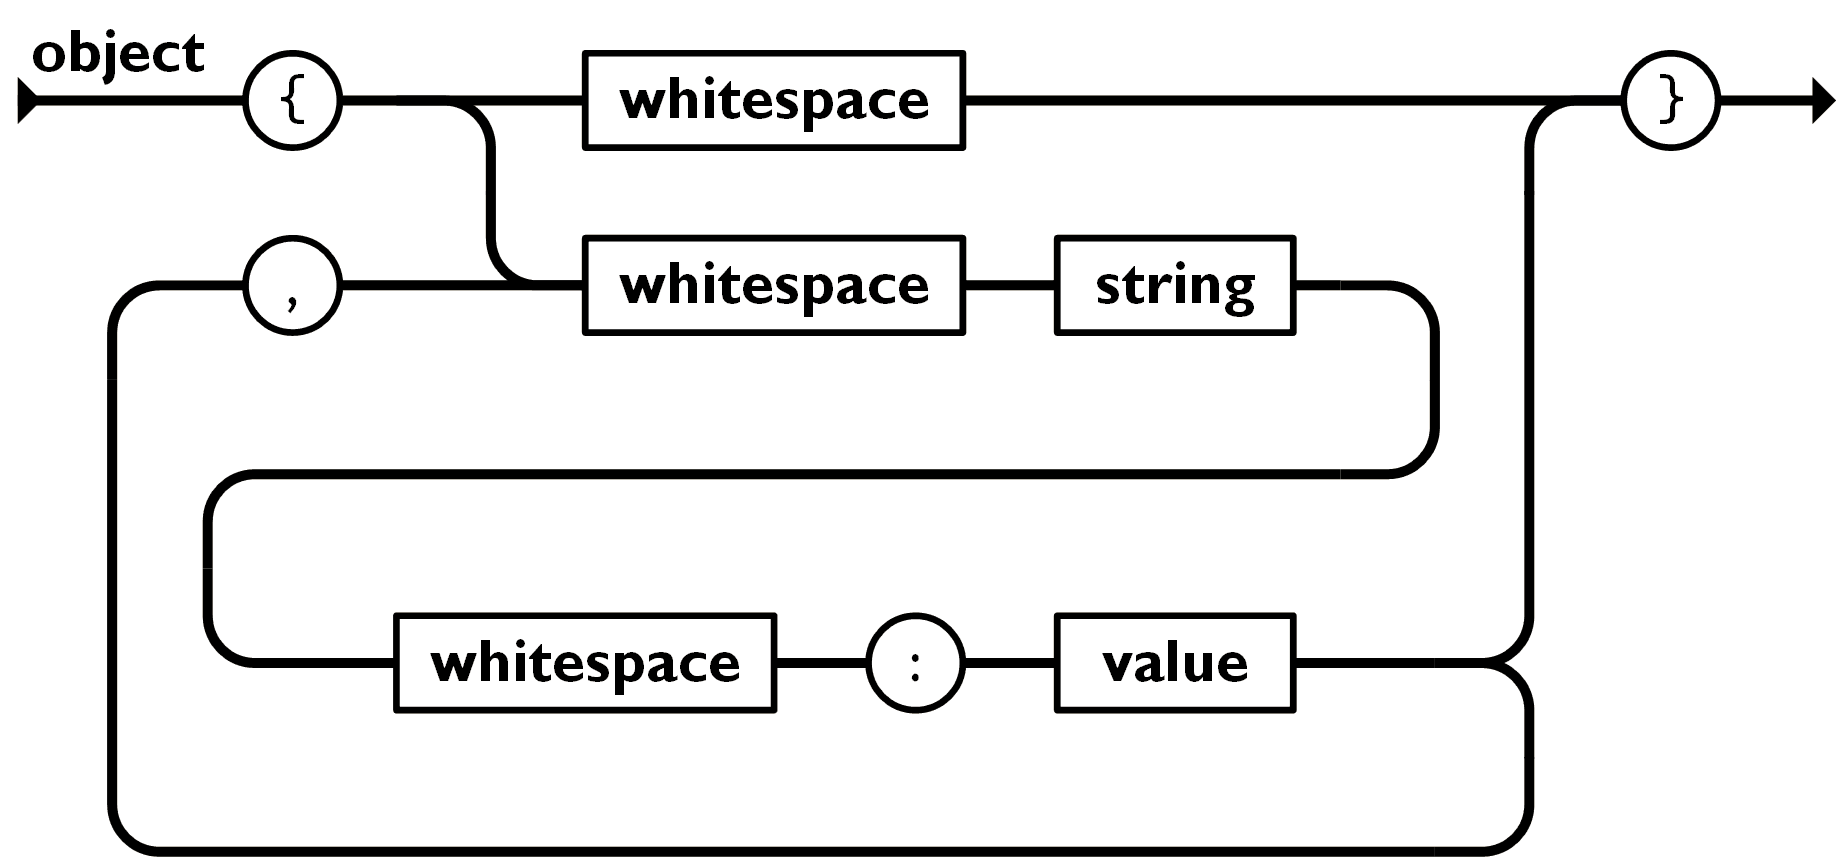
\includegraphics[width=0.9\textwidth]{images/json_object}
        \caption{JSON Object}
        \label{fig:json_object}
    \end{minipage}\hfill
    \begin{minipage}[t]{0.45\textwidth}
        \flushleft\textbf{Array} ist eine geordnete Liste von Values.
        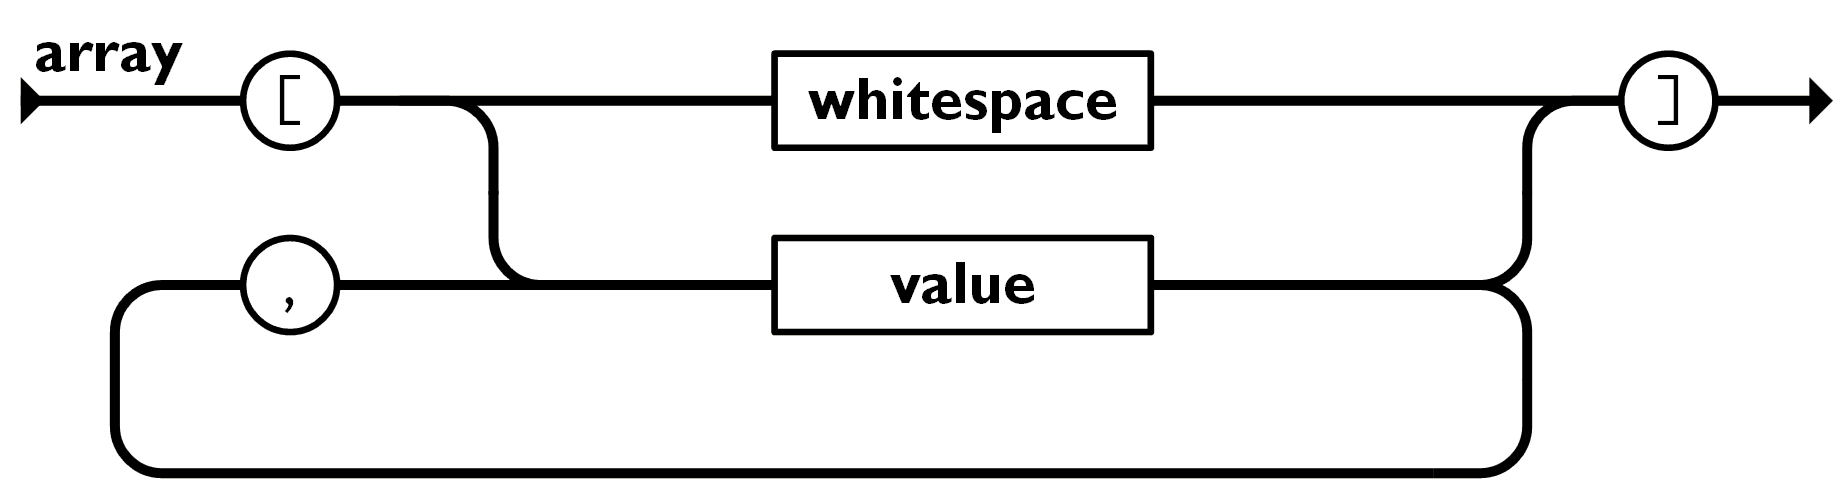
\includegraphics[width=0.9\textwidth]{images/json_array}
        \caption{JSON Array}
        \label{fig:json_array}
    \end{minipage}\hfill
\end{figure}
\begin{figure}[H]
    \begin{minipage}[t]{0.45\textwidth}
        \textbf{Value} kann ein String, eine Zahl, ein Boolean, ein Objekt, ein Array oder null sein.
        Dabei können beliebig viele Values ineinander verschachtelt sein.
        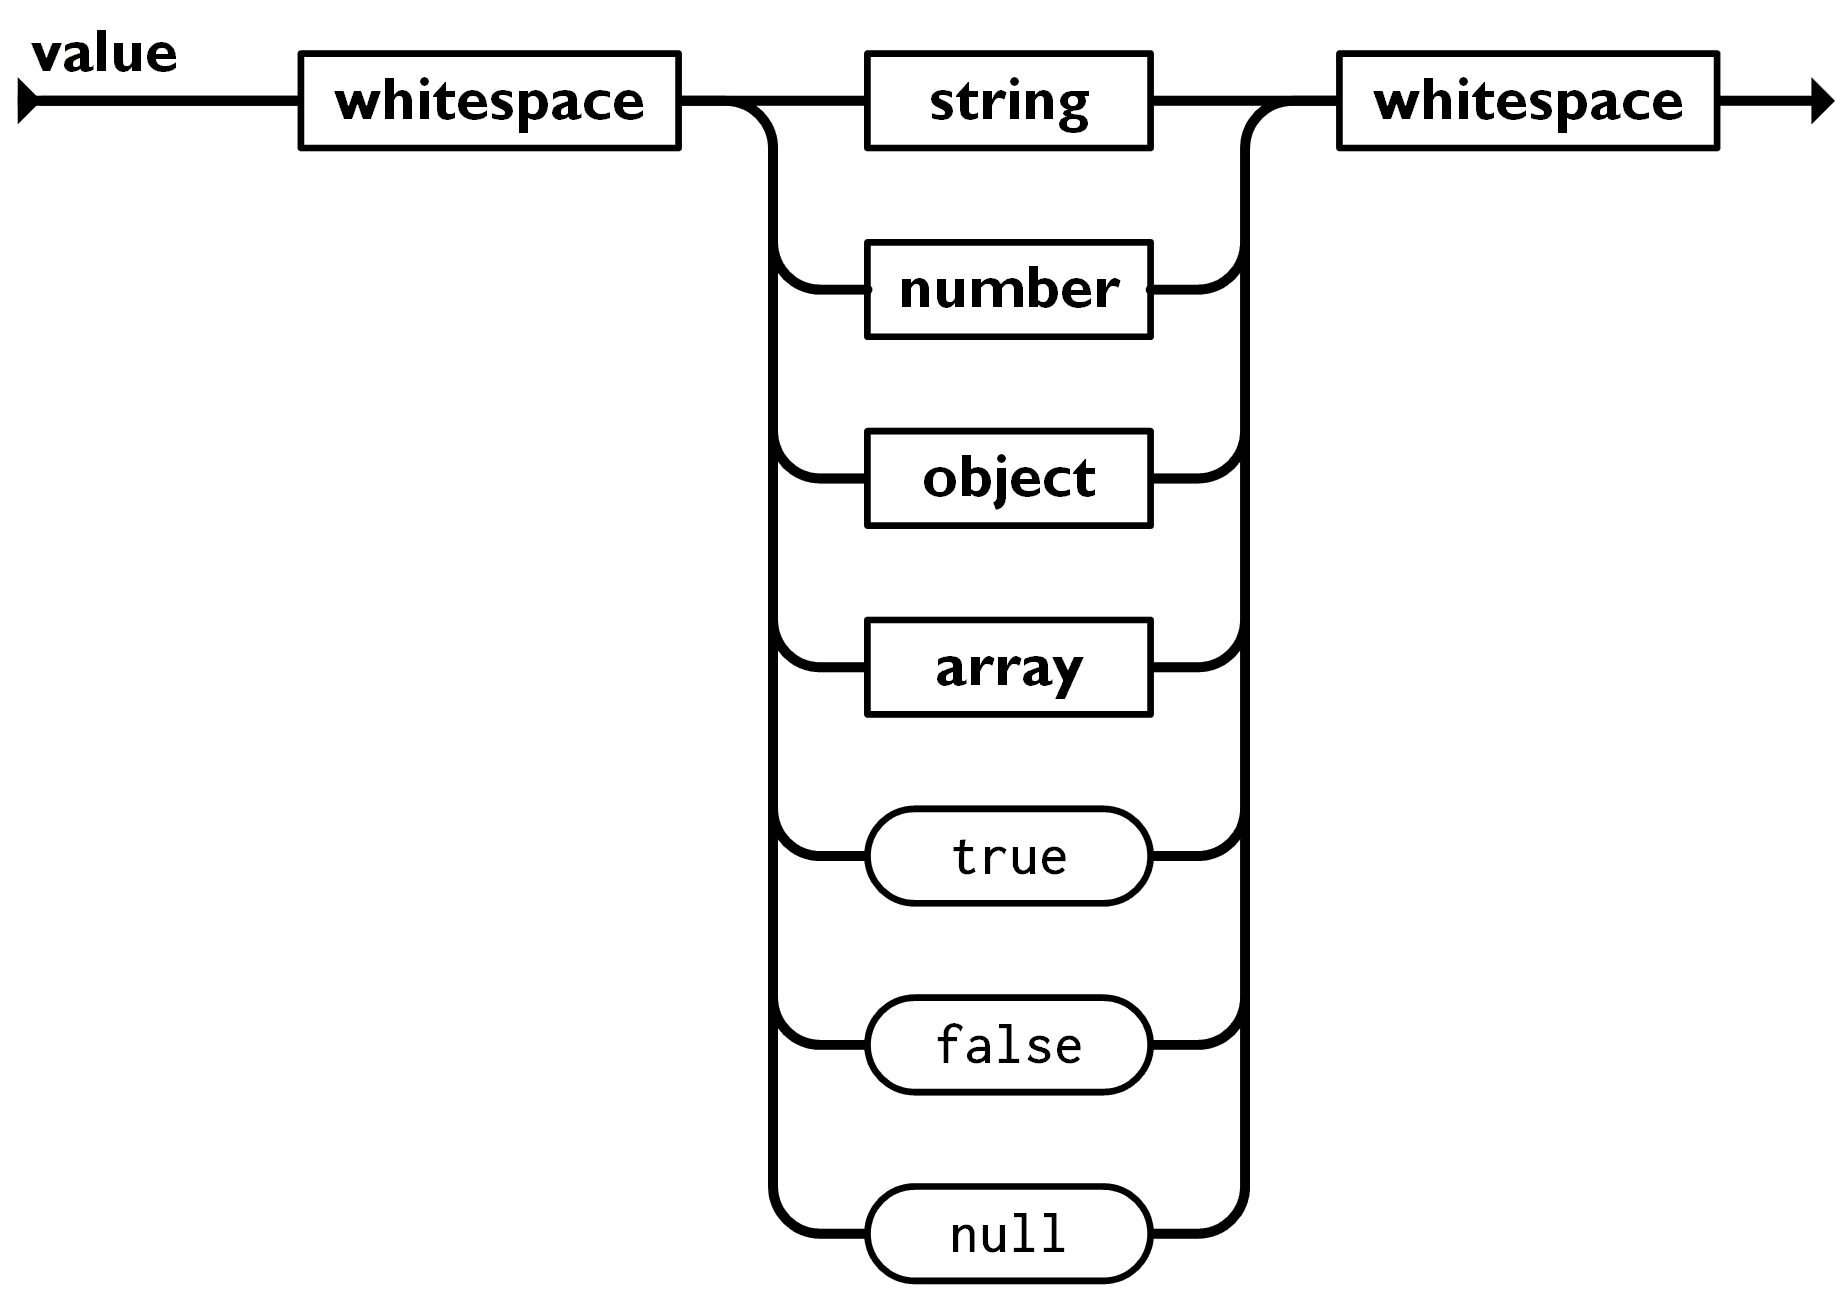
\includegraphics[width=0.9\textwidth]{images/json_value}
        \caption{JSON Value}
        \label{fig:json_value}
    \end{minipage}\hfill
    \begin{minipage}[t]{0.45\textwidth}
        \flushleft\textbf{String} ist eine Sequenz aus Unicode Buchstaben.
        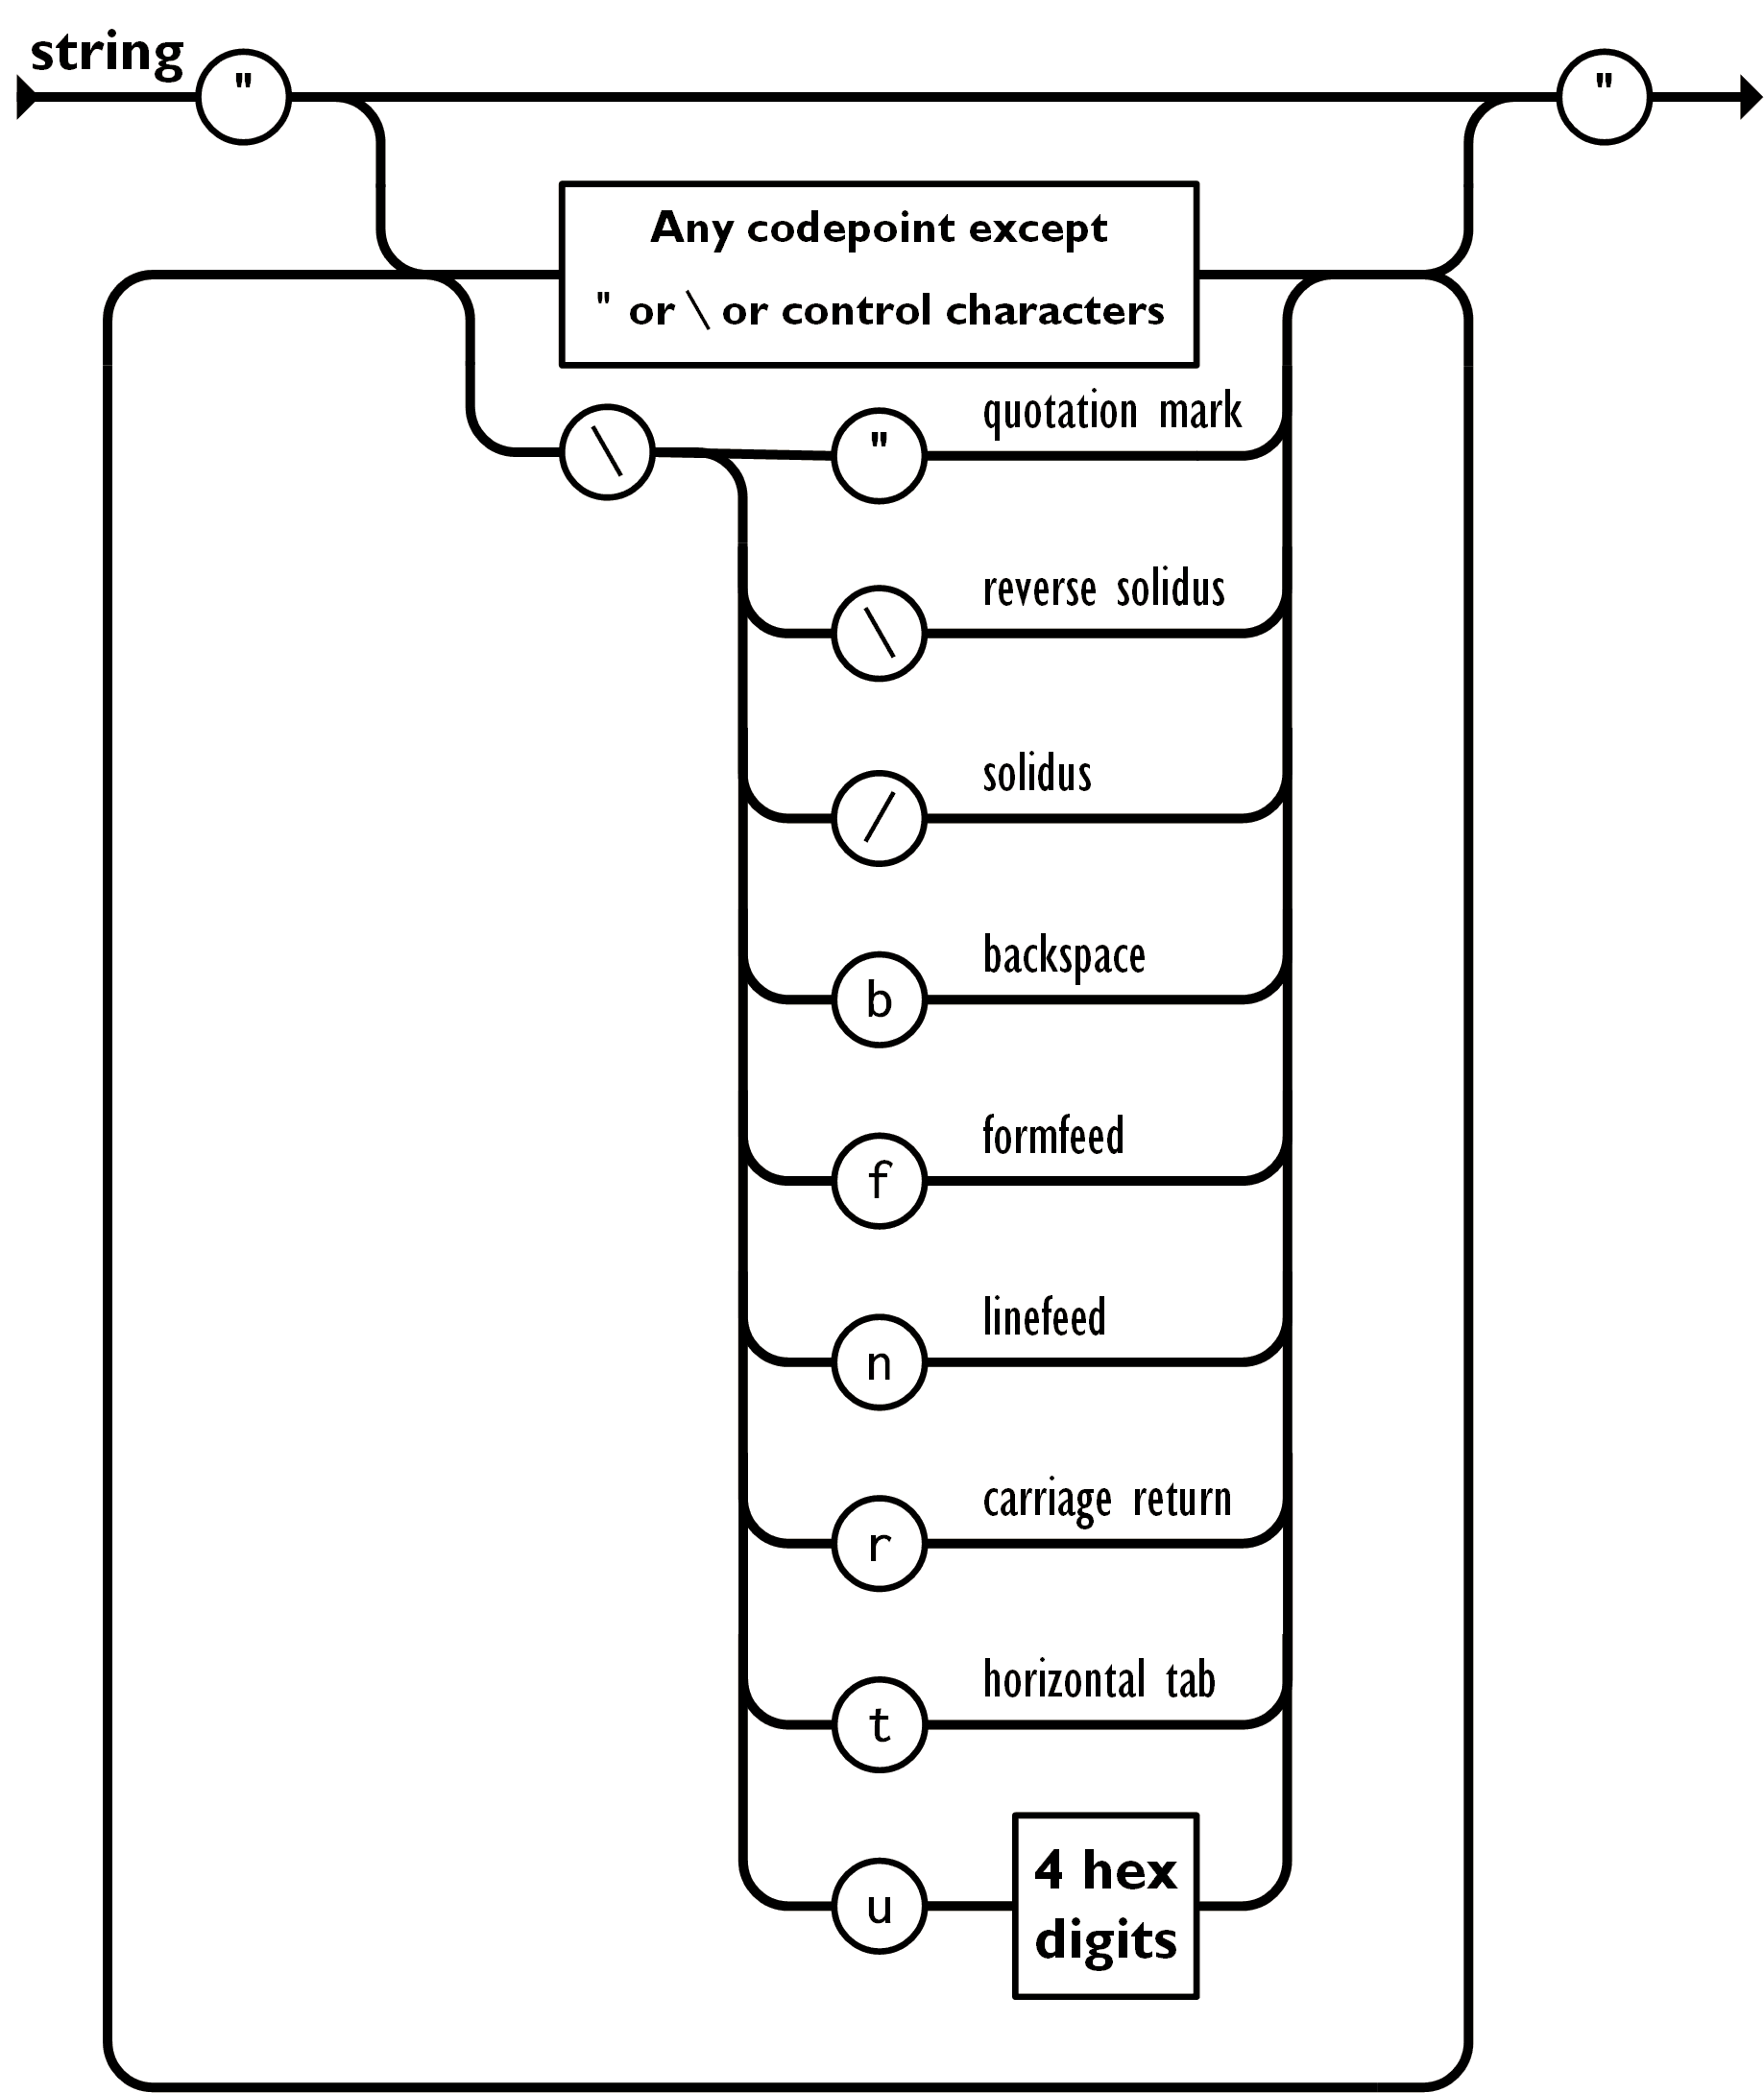
\includegraphics[width=0.9\textwidth]{images/json_string}
        \caption{JSON String}
        \label{fig:json_string}
    \end{minipage}\hfill
\end{figure}
\begin{figure}[H]
    \begin{minipage}[t]{0.45\textwidth}
        \textbf{Number} ist eine Zahl.
        Number kann sowohl eine Gleitkommazahl als auch eine Ganzzahl sein und kann positiv sowie negativ sein.
        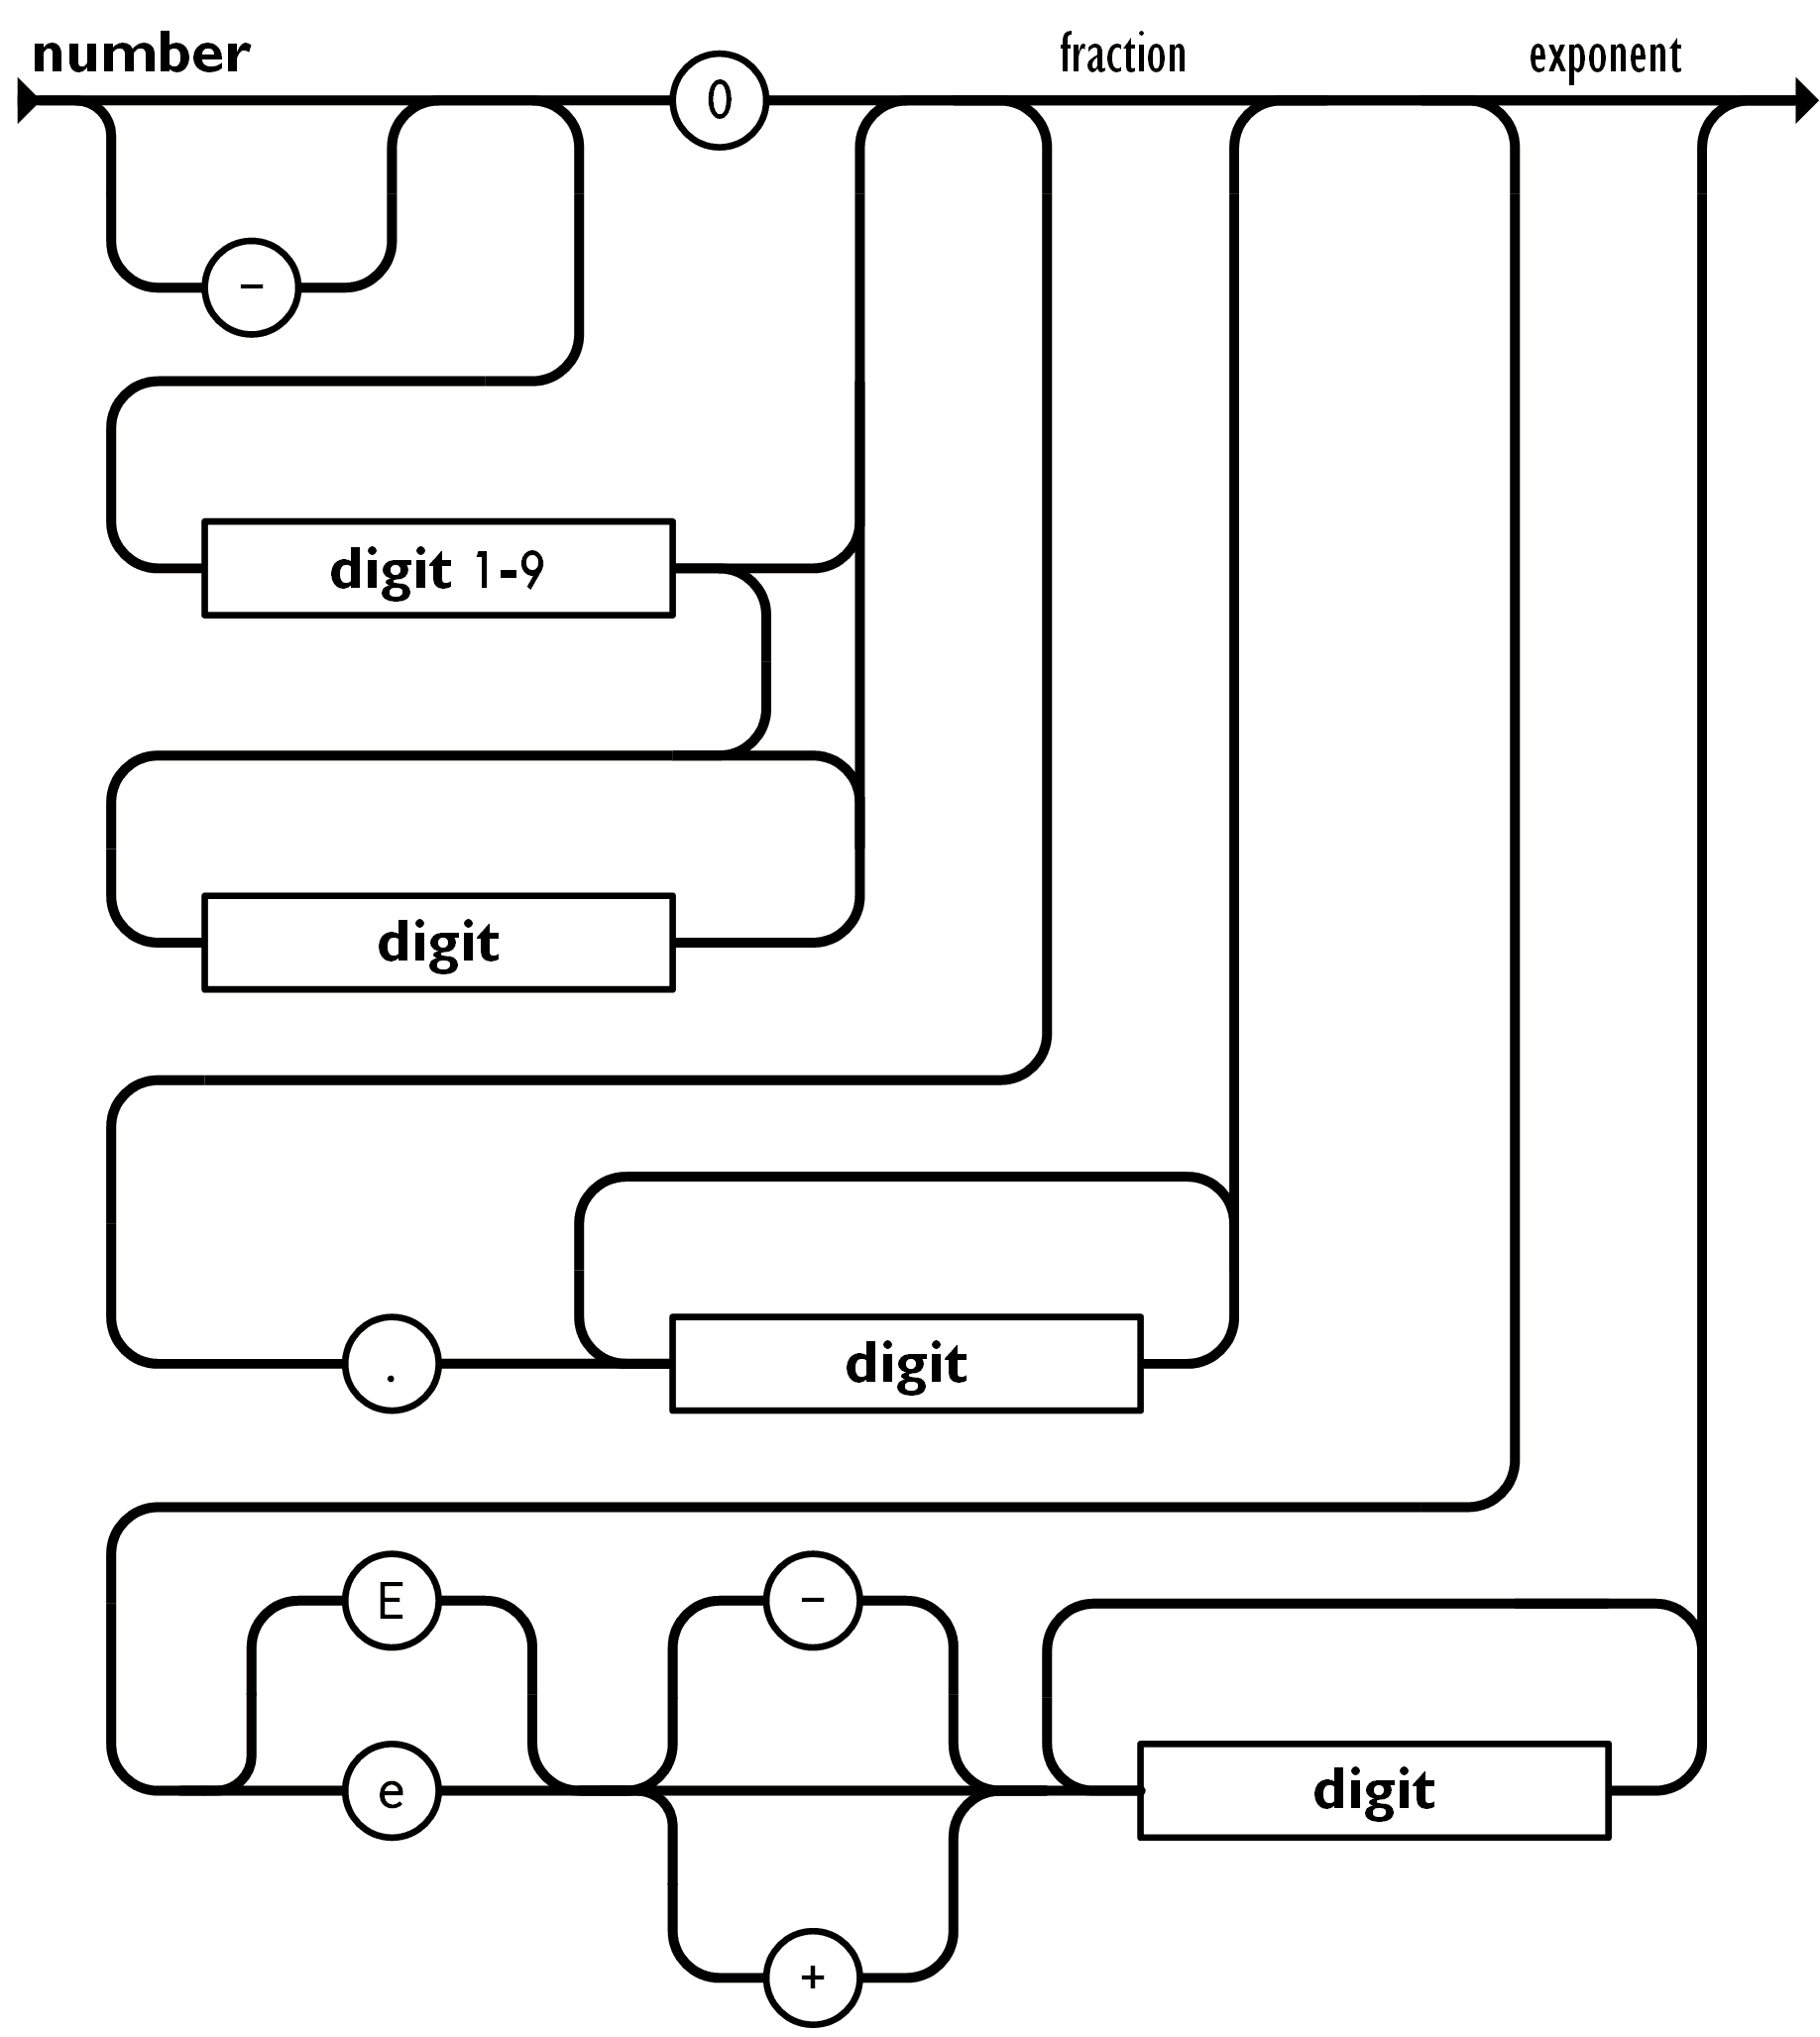
\includegraphics[width=0.9\textwidth]{images/json_number}
        \caption{JSON Number}
        \label{fig:json_number}
    \end{minipage}\hfill
\end{figure}

\section{MongoDB}
\label{sec:mongodb}

MongoDB ist eine Dokument-orientierte Datenbank. 
In Dokument-orientierten Datenbanken wird das aus SQL bekannte Konzept von Reihen durch Dokumente ersetzt.
Dokumente haben im Gegensatz zu Reihen in Tabellen kein fixes Schema, welches sie erfüllen müssen, sondern sind sehr flexibel.
Grundsätzlich bestehen Dokumente aus Key - Value Paaren, welche in einer JSON-Ähnlichen Struktur gespeichert werden.
Dokumente können, wie auch in JSON, ineinander verschachtelt sein, was hierarchische Strukturen und dadurch Denormalisierung ermöglicht.
Die Dokumente werden in Collections organisiert.
Eine Collection entspricht in SQL einer Tabelle ohne das fixe Schema.
Diese Collections befinden sich wiederum in Datenbanken.
Eine MongoDB Instanz kann mehrere voneinander unabhängige Datenbanken beinhalten.
Man kann sich mit der MongoShell mit einer MongoDB Instanz verbinden, um mit der Mongo Query Language oder mit JavaScript die Instanz administrieren und Daten manipulieren zu können.
~\autocite{bradshaw:mongodb}

\section{Python}
\label{sec:python}

Python ist eine objektorientierte high-level Programmiersprache, die besonderen Wert auf Lesbarkeit legt.
Variablen in Python werden dynamisch typisiert.
Das bedeutet, dass eine Variable in Python keinen festen Typ hat, sondern dieser dynamisch über den ihr zugewiesenen Wert bestimmt wird.
Python ist keine kompilierte, sondern eine interpretierte Programmiersprache.
Diese Eigenschaften machen Python zu der idealen Sprache für das Schreiben von Skripten, sowie für Anwendungen, die schnell und simpel entwickelt werden sollen.
PIP ist ein in Python integrierter Paketmanager, der das installieren von Packages erleichtert.
Der Python Interpreter ist in C geschrieben, weshalb man die Funktionalität des Interpreters durch C-Programme erweitern kann, um beispielsweise laufzeitkritische Funktionen in C auszuführen.
~\autocite{van:python}

\section{Flask}
\label{sec:flask}

Flask ist ein minimalistisches Open-Source Web Framework für Python.
In Flask sind ein paar wenige Kernpakete vorinstalliert, welche für ein minimales Backend benötigt werden.
Alles weitere muss der Nutzer selbst über PIP installieren.
~\autocite{grindberg:flask}
Durch diesen minimalistischen Ansatz ist Flask sehr flexibel einsetzbar.
Flask ist beispielsweise mit SQL oder NoSQL Datenbanken, aber auch ganz ohne Datenbanken einsetzbar.

% TODO DOM

\section{JavaScript}
\label{sec:js}

JavaScript ist eine High-Level Programmiersprache, die just-in-time kompiliert wird.
JavaScript ist besonders bekannt als Skriptsprache für Webseiten, wird aber auch für Backendanwendungen, Automatisierungsaufgaben und vieles mehr verwendet.
Die Besonderheit von JavaScript gegenüber anderen Sprachen ist eine vollständige native Kompatibilität und Integration in HTML und CSS.
~\autocite{javascript:javascript}
Die Pakete in JavaScript werden mittels dem Paketmanager NPM verwaltet.

\section{React}
\label{sec:react}

React ist eine JavaScript Bibliothek zum Bauen von Benutzeroberflächen.
React ist Komponentenbasiert.
Das bedeutet, dass React aus einzelnen Komponenten bestehen, die ihren eigenen State haben und die zusammengesetzt ein komplexes \ac{ui} bilden.
~\autocite{banks:react}


\subsection{Redux Store}
\label{sub:redux}

Redux ist ein State Container für JavaScript Apps, der es ermöglicht, States nicht mehr in den einzelnen React Komponenten, sondern in einem zentralen Container zu speichern.
~\autocite{freecodecamp:redux}
Dadurch können States wiederhergestellt werden, nachdem eine Komponente geschlossen und wieder geöffnet wurde.
Außerdem erleichtert Redux es, State Änderungen in Komponenten nachzuvollziehen.

\iffalse
\subsection{Axios}
\label{sub:axios}

Axios ist ein HTTP-Client für JavaScript.
Mithilfe von Axios Können HTTP-Requests versendet und die Responses von diesen verarbeitet werden.
\fi

\section{Docker Container}
\label{sec:docker}

Ein Container ist eine virtuelle Umgebung, die, ähnlich wie eine virtuelle Maschine, eine Anwendung in eine isolierte Umgebung verpackt.
Jedoch wird im Gegensatz zu virtuellen Maschinen nicht das ganze Betriebssystem virtualisiert, sondern nur einzelne Anwendungen.
Dadurch ist ein Container deutlich schlanker als eine virtuelle Maschine.
Container können als sogenannte Images auf verschiedenen Systemen ausgeliefert werden und dabei aufgrund der Isolierung unabhängig vom System zuverlässig funktionieren.
Docker ist eine weit verbreitete Open-Source Software, welche das Container-Prinzip implementiert.
~\autocite{devInsider:container}

\section{Nginx}
\label{sec:nginx}

Nginx, ausgesprochen Engine X, ist ein Open-Source Web Server.
In Nginx sind einige Features für das Hosten von Webservern integriert, wie beispielsweise Load Balancing, Reverse Proxies, Web Sockets, Mail Server und vieles mehr.
Dabei unterstütz Nginx alle gängigen Betriebssysteme, wie Windows, Windows Server, MacOS und Linux.
Die Konfiguration in Nginx erfolgt über Konfigurationsdateien.
Die Nutzung von Nginx als Webserver nimmt jedes Jahr weiter zu im Vergleich zum Kompetitoren wie Apache.
Im Januar 2023 liefen 21,20\% der meistgenutzten Seiten über Nginx.
~\autocite{nginx:nginx}

\section{Microservice Architektur}
\label{sec:microservices}

Die Microservice Architektur ist eine Architektur, bei der das Endprodukt aus einer Sammlung einzelner Services besteht.
Diese Services sind an sich voneinander unabhängig auslieferbar und sind nur lose gekoppelt.
Jeder Service wird von einem einzelnen kleinen Team entwickelt und muss ohne großen Aufwand testbar und wartbar sein.
~\autocite{richardson:microservices}
